 \begin{refsection}
\chapter{Structural basis for gating pore current in periodic paralysis}

The contents of this section were adapted from an article published in the \textit{Nature}.\par
\bigskip
Reference: Jiang, D., Gamal El-Din, T.M., Ing C., Lu, P., Pom\`es, R, Zheng, N., and Catterall, W. A. (2018) Structural basis for gating pore current in periodic paralysis. \textit{Nature}, 557 (7706), 590-594.\par
\bigskip
Contributions: D.J., T.M.G.E.-D., C.I., P.L., R.P., N.Z. and W.A.C. designed experiments. D.J., T.M.G.E.-D., C.I. and P.L. conducted experiments. D.J., T.M.G.E.-D., C.I., R.P., N.Z. and W.A.C. analyzed the results. T.M.G.E.-D., C.I. and W.A.C. wrote the paper with input from all co-authors.

\newpage

\section{Summary}

Potassium-sensitive hypokalaemic and normokalaemic periodic paralysis are inherited skeletal muscle diseases characterized by episodes of flaccid muscle weakness \cite{Venance:2006fc,PMID:28939973}. They are caused by single mutations in positively charged residues (`gating charges') in the S4 transmembrane segment of the voltage sensor of the voltage-gated sodium channel Na\textsubscript{V}1.4 or the calcium channel Ca\textsubscript{V}1.1 \cite{Venance:2006fc,PMID:28939973}. Mutations of the outermost gating charges (R1 and R2) cause hypokalaemic periodic paralysis \cite{Venance:2006fc,PMID:28939973} by creating a pathogenic gating pore in the voltage sensor through which cations leak in the resting state \cite{Sokolov:2007iu,Struyk:2007jp}. Mutations of the third gating charge (R3) cause normokalaemic periodic paralysis \cite{Vicart:2004jh} owing to cation leak in both activated and inactivated states \cite{Sokolov:2008dv}. 

Here we present high-resolution structures of the model bacterial sodium channel Na\textsubscript{V}Ab with the analogous gating-charge mutations \cite{Payandeh:2012ib,Catterall:2015dha}, which have similar functional effects as in the human channels. The R2G and R3G mutations have no effect on the backbone structures of the voltage sensor, but they create an aqueous cavity near the hydrophobic constriction site that controls gating charge movement through the voltage sensor. The R3G mutation extends the extracellular aqueous cleft through the entire length of the activated voltage sensor, creating an aqueous path through the membrane. Conversely, molecular modelling shows that the R2G mutation creates a continuous aqueous path through the membrane only in the resting state. Crystal structures of Na\textsubscript{V}Ab(R2G) in complex with guanidinium define a potential drug target site. Molecular dynamics simulations illustrate the mechanism of Na$^+$ permeation through the mutant gating pore in concert with conformational fluctuations of the gating charge R4. Our results reveal pathogenic mechanisms of periodic paralysis at the atomic level and suggest designs of drugs that may prevent ionic leak and provide symptomatic relief from hypokalaemic and normokalaemic periodic paralysis.
	
\section{Introduction}

Na\textsubscript{V}1.4 channels generate action potentials that initiate muscle contraction \cite{Catterall:2005iw}. They are complexes of a pore-forming $\alpha$-subunit and auxiliary $\beta$1 subunits \cite{Catterall:2005iw,Shen:2017dfa,Yan:2017kda}. The $\alpha$-subunit contains four homologous domains (I-IV), each with six transmembrane segments (S1-S6). Segments S1-S4 form the voltage sensor, and every third residue in S4 is positively charged. Upon depolarization, S4 moves outward through a narrow gating pore formed by S1-S3, catalysed by interactions with negative or polar residues in S2 and S3 \cite{Catterall:2010kra}. The voltage sensor has an hourglass shape, with a narrow hydrophobic constriction site (HCS) that separates extracellular and intracellular compartments \cite{Payandeh:2012ib,Shen:2017dfa}. Water-filled crevices on either side of the HCS focus the membrane electric field, assuring efficient coupling of voltage to conformational changes that open the central pore \cite{Catterall:2010kra,Starace:2004ea}. Mutations in the arginine gating charges that occupy the HCS cause state-dependent cation leak through the voltage sensor, which we term `gating pore current' \cite{GamalElDin:2014gu,Sokolov:2010ii}.

Missense mutations of arginine gating charges in S4 of Na\textsubscript{V}1.4 cause hypokalaemic periodic paralysis and normokalaemic periodic paralysis \cite{PMID:28939973,JurkatRott:2012kv,Moreau:2014jy,Venance:2006fc}. Mutations of R1 in domains I or III to H or Q, or mutation of R2 in domains I, II and III to W, G, Q or S cause hypokalaemic periodic paralysis \cite{PMID:28939973,JurkatRott:2012kv,Moreau:2014jy,Venance:2006fc}. Mutations of R3 in domain II to G, Q or W, or of R3 in domain III to H or C cause normokalaemic periodic paralysis \cite{JurkatRott:2012kv,Moreau:2014jy,Struyk:2007jp}. All these mutations result in non-selective gating pore current through the voltage sensor \cite{JurkatRott:2012kv,Moreau:2014jy,Sokolov:2007iu,Struyk:2007jp,Wu:2012fj,Wu:2011il}. Increased inward leak leads to Na$^+$ overload, sustained depolarization and action potential failure, which paralyze skeletal muscles \cite{JurkatRott:2012kv,Moreau:2014jy,Sokolov:2007iu,Wu:2012fj,Wu:2011il}. These pathophysiological effects suggest that mutations that cause hypokalaemic periodic paralysis result in an open aqueous pathway for ion movement in the resting state of the voltage sensor, but not in the activated state, and mutations that cause normokalaemic periodic paralysis result in an open aqueous pathway in the activated state, but not in the resting state. Molecular models and mutagenesis studies support this hypothesis \cite{GosselinBadaroudine:2012eh,Monteleone:2017gj,Moreau:2015je}. To provide direct structural evidence for this pathophysiological mechanism, we introduced mutations known to cause periodic paralysis into Na\textsubscript{V}Ab, a voltage-gated Na$^+$ channel from Arcobacter butzleri, the structure of which has been solved at high resolution \cite{Payandeh:2012ib}. We characterized the resulting gating pore currents, solved the structures of mutant gating pores without and with a bound permeant ion, and investigated molecular dynamics \cite{Chakrabarti:2013kd} of ion movement through the gating pores.

\section{Results}

Pathogenic hypokalaemic periodic paralysis gating pore currents were reconstituted in Na\textsubscript{V}Ab by mutating R2 to S (R2S, analogous to Na\textsubscript{V}1.4(R672S)) \cite{Jiang:2018ga}. Electrophysiological measurements confirm a nonlinear leak current component in the resting state of the channel. Mutations of the gating charge R3 that cause normokalaemic periodic paralysis (Nav\textsubscript{V}1.4(R675G/Q/W)) induce outward gating pore current in activated but not in resting states. Na\textsubscript{V}Ab(R3G) conducted outward gating pore current in both activated and inactivated states \cite{Jiang:2018ga}. These physiological studies demonstrate that Na\textsubscript{V}Ab provides an accurate model of Na\textsubscript{V}1.4, because gating pore current is observed only in the resting state for Na\textsubscript{V}Ab(R2S) and only in the activated and inactivated states for Na\textsubscript{V}Ab(R3G).

%To reconstitute pathogenic hypokalaemic periodic paralysis gating pore currents in Na\textsubscript{V}Ab, we mutated R2 to S (R2S, analogous to Nav\textsubscript{V}1.4(R672S)) and expressed the mutant in Trichopulsiani insect cells. Transfected cells were voltage-clamped to ?200 mV and depolarized in 10-mV steps to record Na$^+$ currents. Half-maximal activation of central pore currents was observed at Va = ?105 � 0.6 mV (Fig. 1a). To measure gating pore currents, cells were held at ?100 mV, at which Na\textsubscript{V}Ab is in the slow-inactivated state and exhibits no central pore current. Gating pore current was examined by applying pulses from + 100 to ?200 mV in ?10 mV steps. A nonlinear leak current component was observed in the resting state, beginning at ?110 mV and increasing to ?200 mV (Fig. 1b, c).

%Mutations of the gating charge R3 that cause normokalaemic periodic paralysis (Nav\textsubscript{V}1.4(R675G/Q/W)) induce outward gating pore current in activated but not in resting states6. In Na\textsubscript{V}Ab(R3G), central pore current was activated between ?50 mV and 0 mV (Fig. 1d; Va = ?24.8 � 1.1 mV). Steady-state inactivation was observed from ?90 mV to ?10 mV with half maximal inactivation at Vh = ?47.7 � 0.4 mV (Fig. 1d). Na\textsubscript{V}Ab(R3G) conducted outward gating pore current in both activated and inactivated states at potentials more positive than ?60 mV (Fig. 1e, f ). These physiological studies demonstrate that Na\textsubscript{V}Ab provides an accurate model of Nav\textsubscript{V}1.4, because gating pore current is observed only in the resting state for Na\textsubscript{V}Ab(R2S) and only in the activated and inactivated states for Na\textsubscript{V}Ab(R3G).

The pathogenic effects of gating pore mutations depend on inward leak of Na$^+$. The R2S mutant gating pore was not significantly selective among Cs$^+$, K$^+$ or Na$^+$ \cite{Jiang:2018ga}. As is the case for Nav\textsubscript{V}1.424, the gating pore of Na\textsubscript{V}Ab(R2S) was exceptionally permeant to guanidinium (about 28-fold greater than Na$^+$), but it was less permeant to methyl-guanidinium and ethylguanidinium \cite{Jiang:2018ga}. The outward gating pore currents conducted by Na\textsubscript{V}Ab(R3G) were higher for Cs$^+$ than for K$^+$ or Na$^+$, which were similar to each other. However, Na\textsubscript{V}Ab(R3G) was less permeant to guanidinium than to Na$^+$, and it was more than 16-fold less permeant to guanidinium than Na\textsubscript{V}Ab(R2S) \cite{Jiang:2018ga}. The weak selectivity of R2S and R3G mutants for different inorganic cations and the high guanidinium permeability through the R2S mutant are characteristic of the corresponding mutations in Na\textsubscript{V}1.4 2, further supporting the validity of Na\textsubscript{V}Ab as a model for structural studies of gating pore mutations.

To elucidate the structure of a pathogenic gating pore in its conductive conformation in an activated voltage sensor, we solved the structure of a Na\textsubscript{V}Ab analogue of a normokalaemic periodic paralysis-causing mutation, Na\textsubscript{V}Ab(R3G), at 2.7 \AA resolution (Fig. \ref{fig:navVSDfig2}). Voltage-gated sodium channels have a central pore module surrounded by four symmetrically located voltage sensors (Fig. \ref{fig:navVSDfig2} A). The voltage sensors of Na\textsubscript{V}Ab and Na\textsubscript{V}1.4 are very similar in amino acid sequence and structure. The voltage sensors of wild-type (WT) Na\textsubscript{V}Ab and Na\textsubscript{V}Ab(R3G) crystallize in the same conformation, with a C$\alpha$ root mean square deviation (r.m.s.d.) of 0.39 \AA (Fig. \ref{fig:navVSDfig2} B). These results indicate that the R3G mutation does not perturb the overall structure of the voltage sensor and, therefore, that its pathogenic effects are caused by the loss of the R3 side chain. These channels crystallize with an activated voltage sensor \cite{Payandeh:2012ib} (Fig. \ref{fig:navVSDfig2} C), as would be expected at 0 mV. In Na\textsubscript{V}Ab(WT), R1, R2 and R3 are located extracellularly relative to the HCS, and their side chains point outward, toward the extracellular milieu (Fig. \ref{fig:navVSDfig2} C). By contrast, R4 is located intracellularly relative to the HCS and its side chain points inward towards the cytosol (Fig. \ref{fig:navVSDfig2} C). When viewed from the extracellular side, there is no water-accessible path into the cell through the wild-type voltage sensor (Fig. \ref{fig:navVSDfig2} D); however, we observed a deep solvent-accessible cleft extending down to the R4 side chain in Na\textsubscript{V}Ab(R3G) (Fig. \ref{fig:navVSDfig2} G).

\begin{figure}[!ptb]
\centering
\includegraphics[width=0.7\textwidth]{navvsd/NavVSDFig2}
\caption[Structures of the voltage sensor of Na\textsubscript{V}Ab(WT) and Na\textsubscript{V}Ab(R3G)]{\textbf{Structures of the voltage sensor of Na\textsubscript{V}Ab(WT) and Na\textsubscript{V}Ab(R3G)}. (\textbf{A}) Structure of Na\textsubscript{V}Ab(R3G) in top view. (\textbf{B}) Comparison of the conformations of Na\textsubscript{V}Ab(WT) (grey) and Na\textsubscript{V}Ab(R3G) (rainbow) voltage sensor in side view. (\textbf{C-E}) Structures of Na\textsubscript{V}Ab(WT) voltage sensor. (\textbf{C}) Side view highlighting gating charges in sticks. (\textbf{D}) Top view in space-filling format. (\textbf{E}) MOLE2 analysis of water-accessible space
in magenta. (\textbf{F-H}) Structures of Na\textsubscript{V}Ab(R3G) voltage sensor. (\textbf{F}) Side view highlighting gating charges. (\textbf{G}) Top view in space-filling format. (\textbf{H}) MOLE2 analysis of water-filled space in magenta. Green spheres in \textbf{F} and \textbf{H} indicate the positions of the missing side chain of R3. In \textbf{D} and \textbf{G}, the dotted red line circles the position where the gating pore would be in the activated state and the solid red line circles the open gating pore, respectively.}
\label{fig:navVSDfig2}
\end{figure}

Analysis of the structure of chain B of Na\textsubscript{V}Ab(WT) using the MOLE2 algorithm revealed an incomplete water-accessible path extending part of the way through the voltage sensor from both extracellular and intracellular sides, which is interrupted at the HCS by R3 (Fig. \ref{fig:navVSDfig2} E). Strikingly, in Na\textsubscript{V}Ab(R3G), the water-accessible path continues all the way through the voltage sensor, and has a diameter of 2 \AA at its narrowest point, similar to the size of Na$^+$ (Fig. \ref{fig:navVSDfig2} H). By contrast, in chain A, R4 was captured in a rotamer conformation in which the arginine side chain partially blocks the inner end of the gating pore in Na\textsubscript{V}Ab(R3G). Previously reported structures of Na\textsubscript{V}Ab in the slow-inactivated state show that R4 adopts four slightly different rotamer conformations, with the most open having a diameter of 3 \AA \cite{Payandeh:2012ex}. These results elucidate the molecular mechanism by which mutations in S4 cause pathogenic gating pore currents and suggest that ion permeation through the gating pore is controlled dynamically by the state of the voltage sensor and by rotamer conformations of R4.

In contrast to voltage-gated sodium-channel mutations that cause normokalaemic periodic paralysis, those that cause hypokalaemic periodic paralysis result in a channel that conducts gating pore current in the resting state but is closed in the activated state. Therefore, we hypothesized that Na\textsubscript{V}Ab(R2G) would not have a continuous water-accessible path through its gating pore in the activated state. Analysis of the 2.9 \AA structure of Na\textsubscript{V}Ab(R2G) revealed a gap with additional solvent-accessible area in the extracellular aqueous cleft in comparison to the wild-type channel, but no change in the backbone conformation (Fig. \ref{fig:navVSDfig3} A). Although the increased opening of the aqueous cleft in the voltage sensor is evident in space-filling models (Fig. \ref{fig:navVSDfig3} B), the R3 and R4 side chains seal the voltage sensor in this activated state, interrupting the transmembrane path and preventing ion conductance. The solvent-accessible area penetrates about 21 \AA into the membrane from the extracellular side (Fig. \ref{fig:navVSDfig3} C), more than 7 \AA deeper than in Na\textsubscript{V}Ab(WT) (Fig. \ref{fig:navVSDfig2} E), but it does not reach the cytosolic side. This structure illustrates why Na\textsubscript{V}Ab(R2G) does not conduct gating pore current in the activated state.

\begin{figure}[!ptb]
\centering
\includegraphics[width=0.7\textwidth]{navvsd/NavVSDFig3}
\caption[Structure of voltage sensor and guanidinium binding site of Na\textsubscript{V}Ab(R2G)]{\textbf{Structure of voltage sensor and guanidinium binding site of Na\textsubscript{V}Ab(R2G)}. (\textbf{A-C}) Structures of the activated voltage sensor of Na\textsubscript{V}Ab(R2G). (\textbf{A}) Side view with gating charges highlighted in sticks. (\textbf{B}) Top view in space-filling format. The dashed red line indicates the position of the closed gating pore. (\textbf{C}) MOLE2 analysis of water-filled space in magenta. (\textbf{D-F}) Rosetta structural models of resting state 2 of the voltage sensor were reoptimized with the amino-acid sequence of Na\textsubscript{V}Ab for Na\textsubscript{V}Ab(WT). (\textbf{D}) Na\textsubscript{V}Ab(R2G) (\textbf{E}) and Na\textsubscript{V}Ab(R3G). (\textbf{F}) The perspective is rotated approximately 180 degrees around the vertical axis to better illustrate the arginine gating charges in resting state 2. Green spheres represent missing arginine side chains of R2 and R3, respectively. Magenta blobs represent solvent- accessible volume modelled with MOLE2. (\textbf{G}) Top view of Na\textsubscript{V}Ab(R2G) with one guanidinium bound to each voltage sensor. (\textbf{H}) 2mFo-DFc electron density map (blue mesh) of residues around the guanidinium binding site at 1$\sigma$. (\textbf{I}) Interaction network between guanidinium and amino acids in the voltage sensor of Na\textsubscript{V}Ab(R2G). Grey dashed lines show interatomic distances shorter than 4 \AA.}
\label{fig:navVSDfig3}
\end{figure}

There are no crystal structures of the voltage sensor of a voltage-gated sodium channel in the resting state, because the resting state is only accessible at negative membrane potentials. However, we developed models of three resting states using disulfide locking of substituted cysteine residues and structure prediction with the Rosetta algorithm \cite{YarovYarovoy:2012et}; these are now considered consensus models of the actual resting states \cite{Catterall:2017if,Vargas:2012eka}. To model an open gating pore with the voltage sensor in the resting state, we introduced the R2G and R3G mutations into these resting-state models and analysed the resulting structures with the MOLE2 algorithm (Fig. \ref{fig:navVSDfig3} D-F). There is no continuous path through the voltage sensor in the wild-type resting-state structure (Fig. \ref{fig:navVSDfig3} D), whereas the resting state of the Na\textsubscript{V}Ab(R2G) voltage sensor contains a continuous water-accessible path through the membrane (Fig. \ref{fig:navVSDfig3} E). Loss of the R2 side chain leaves a gap at the HCS that is large enough for Na$^+$ to pass through (Fig. \ref{fig:navVSDfig3} E). By contrast, the transmembrane pathway is incomplete in Na\textsubscript{V}Ab(R3G) because the R2 side chain occupies the HCS and blocks the gating pore (Fig. \ref{fig:navVSDfig3} F). These structural models illustrate how R2 charge mutations that cause hypokalaemic periodic paralysis result in gating pore current in the resting state.

The Na\textsubscript{V}Ab(R2S) mutant channel is much more permeant than Na\textsubscript{V}Ab(R3G) to guanidinium ions \cite{Jiang:2018ga,Sokolov:2010ii}. Guanidinium ions are chemically similar to the distal moiety of the arginine side chain, and guanidine compounds with hydrophobic substituents can block mutant gating pores \cite{Sokolov:2010ii}. We probed our gating pore structures for guanidinium-binding sites by soaking crystals of Na\textsubscript{V}Ab(R2G) and Na\textsubscript{V}Ab(R3G) with guanidinium and methylguanidinium to determine whether they would bind in place of the missing side chain of R2 or R3. The crystal structures did not show guanidinium binding to Na\textsubscript{V}Ab(R3G). However, crystals of Na\textsubscript{V}Ab(R2G) soaked with guanidinium or methyl-guanidinium diffracted to 2.7 \AA and 2.5 \AA resolution, respectively, and unambiguous electron density was observed in place of each R2 side chain (Fig. \ref{fig:navVSDfig3} G-I). Bound guanidinium is clearly seen in 2Fo-Fc maps (Fig. \ref{fig:navVSDfig3} H). E32 and M29 from S1, N49 from S2, R1 and R3 from S4, and Q150 from an adjacent subunit form the binding site for guanidinium (Fig. \ref{fig:navVSDfig3} I). M29 and R3 each bind guanidinium through hydrogen bonds (Fig. \ref{fig:navVSDfig3} H,I). The carbonyl group of E32 and the carbonyl oxygen of R1 further lock guanidinium in place (Fig. \ref{fig:navVSDfig3} H,I). The binding site is flanked by hydrogen bonds from N49 and Q150 that stabilize guanidinium from opposite sides (Fig. \ref{fig:navVSDfig3} H,I). The binding site for methylguanidinium is almost identical. These structures capture guanidinium bound at a specific site in the closed R2G gating pore. The amino acid residues responsible for guanidinium binding are highly conserved in Na\textsubscript{V}Ab, Na\textsubscript{V}1.4 and Ca\textsubscript{V}1.1. Substituted guanidinium ions can block gating pore current without major effects on Na\textsubscript{V}1.4 function \cite{Sokolov:2010ii}, suggesting that guanidinium-containing compounds specific for this binding site could provide a basis for structure-based drug design and be used therapeutically to relieve the symptoms of hypokalaemic periodic paralysis.

To examine relationships among structural fluctuations of the gating pore, ionic hydration and Na$^+$ leakage, we performed molecular dynamics simulations of wild-type and R3G mutant voltage sensors in a hydrated lipid bilayer (Fig. \ref{fig:navVSDfig4}). Multiple unbiased simulation repeats, with a total duration of 30 $\mu$s, show that the overall structures are conserved. Analysis of axial distributions of water molecules revealed a narrow region (-5 \AA < z < 5 \AA) that is more hydrated in the R3G mutant than in the wild-type voltage sensor, owing to the larger size of the lumen in the mutant (Fig. \ref{fig:navVSDfig4} A-C, yellow; P < 0.002). The average count of water molecules within the HCS was $3.9 \pm 0.8$ and $5.3 \pm 0.4$ for the wild type and R3G mutant, respectively (Fig. \ref{fig:navVSDfig4} E). We performed umbrella sampling simulations to compute the free energy of Na$^+$ permeation along the principal axis of the voltage sensor. When Na$^+$ was within the HCS, the number of water molecules in the HCS increased to $8.4 \pm 0.3$ in the wild type and $9.0 \pm 0.3$ in the R3G mutant, respectively. The free-energy profile for Na$^+$ translocation forms a broad barrier spanning the HCS, centred at C$\alpha$ of R3. The R3G mutation significantly decreases the height of this barrier from $18 \pm 0.8$ to $11 \pm 1.4$ kcal mol$^{-1}$ (Fig. \ref{fig:navVSDfig4} E). These values are consistent with the undetectable gating-pore conductance in the wild type and an upper limit of around 0.1 pS in the R3G mutant \cite{Cooper:1988gh}. Analysis of ionic coordination shows that, at the extracellular edge of the barrier, the first solvation shell of Na$^+$ is almost exclusively composed of water, consistent with the hydrophobic nature of the bottleneck in the voltage sensor (Fig. \ref{fig:navVSDfig4} F). The total coordination number of $5.81 \pm 0.02$ in bulk water drops to $4.88 \pm 0.04$ at the peak of the free-energy barrier, suggesting a large desolvation penalty for Na$^+$ that is partly alleviated by the cavity created in the absence of the R3 side chain. Charge-charge repulsion is also likely to contribute substantially to the higher energy barrier to Na$^+$ permeation in the wild type, impeding the gating pore leakage observed in the R3G mutant.

\begin{figure}[!ptb]
\centering
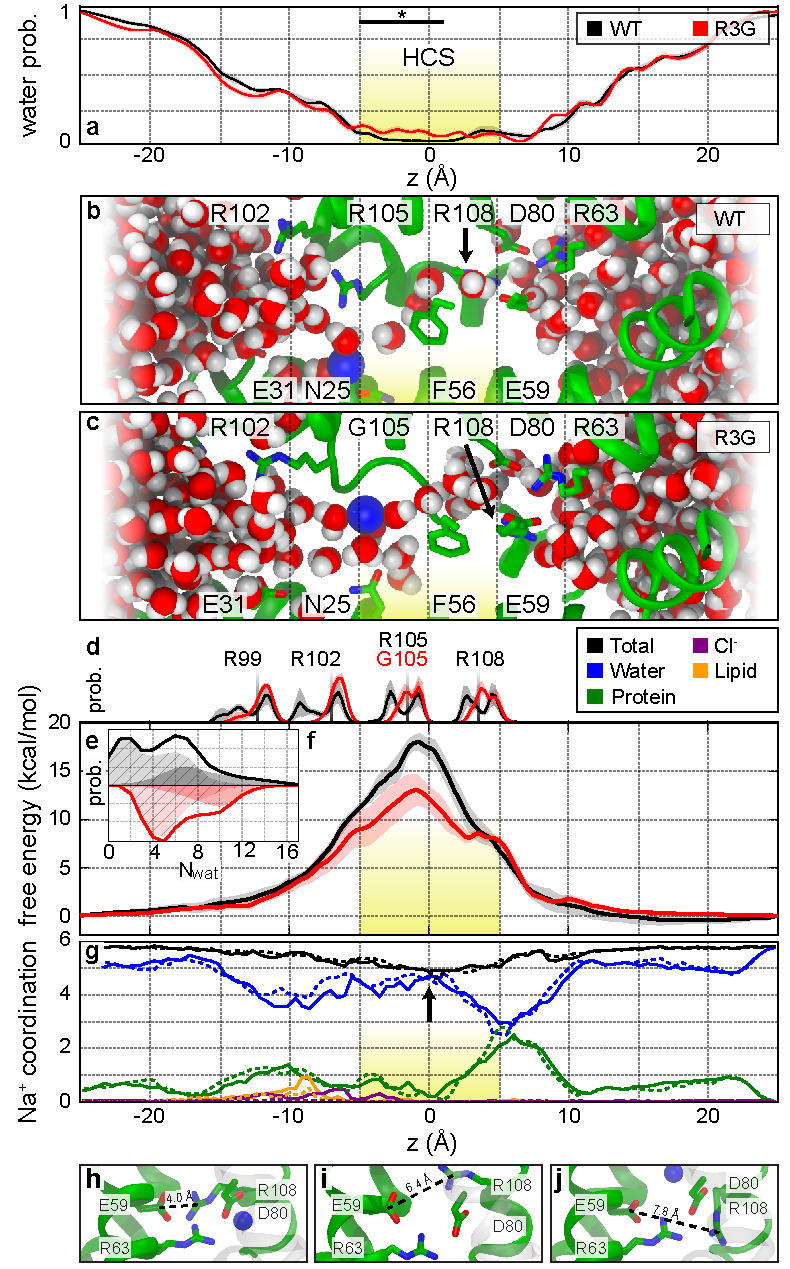
\includegraphics[width=0.5\textwidth]{navvsd/NavVSDFig4}
\caption[R3G mutation lowers the free-energy barrier for Na$^+$ conductance]{\textbf{R3G mutation lowers the free-energy barrier for Na$^+$ conductance}. (\textbf{A}) Probability (prob.) distribution of water along the domain axis for Na\textsubscript{V}Ab(WT) (black) and Na\textsubscript{V}Ab(R3G) (red). (\textbf{B-C}) Representation of voltage sensor from Na\textsubscript{V}Ab(WT) and Na\textsubscript{V}Ab(R3G) simulations where Na$^+$ (blue sphere) is restrained at z = -5 \AA. The S2 segment (residues 45-65) is omitted for clarity. Arrows indicate the positions of R108. (\textbf{D}) Axial distribution of gating charge C$\alpha$ for Na\textsubscript{V}Ab(WT) and Na\textsubscript{V}Ab(R3G). The axial position in the crystallographic structure is shown as a vertical line. (\textbf{E}) Inset, probability distribution of water in the HCS (-5 \AA to 5 \AA) across all simulations of Na\textsubscript{V}Ab(WT) (black) and Na\textsubscript{V}Ab(R3G) (red). The total probability is separated into frames where Na$^+$ occupies the hydrophobic constriction (solid) or is outside this region (cross-hatched). $N_{wat}$, number of water molecules. Main panel, Potential of mean force for Na$^+$ conduction within the Na\textsubscript{V}Ab(WT) (black) and Na\textsubscript{V}Ab(R3G) (red) pore computed using umbrella sampling. The HCS is highlighted in yellow. (\textbf{F}) Average coordination of Na$^+$ as a function of ionic position along the principal axis of the voltage sensor, for Na\textsubscript{V}Ab(WT) (solid lines) and Na\textsubscript{V}Ab(R3G) (dashed lines). The first coordination shell of Na$^+$ is partitioned for coordination to protein (green), water (blue), lipid head groups (orange) and counterions (purple). (\textbf{G-I}) Representative snapshots from simulations of Na\textsubscript{V}Ab(R3G) depicting conformational isomerization of R4. *P < 0.002, n = 60. Arrow in g indicates the point of minimum coordination of Na$^+$ by water.}
\label{fig:navVSDfig4}
\end{figure}

The location of R4 coincides with a secondary shoulder in the free-energy profiles (Fig. \ref{fig:navVSDfig4} D, R108), indicating that movement of Na$^+$ past R4 is not rate-limiting for permeation, even though transit of Na past R4 causes the largest displacement of water by protein ligands (Fig. \ref{fig:navVSDfig4} E). Spontaneous disruption of the R4-E59 salt bridge in $3 \pm 1$\% of simulation frames for the wild type and R3G mutant opens the inner end of the gating pore with sufficient frequency to support gating pore current (Fig. \ref{fig:navVSDfig4} G-I). Na$^+$ often makes direct contacts with the anionic side chains of D80 and E59 (Fig. \ref{fig:navVSDfig4} F,G), and its movement is coupled to dynamic rearrangements of the R4 salt-bridge network.

\section{Discussion}
Overall, our results provide an unprecedented high-resolution view of functional effects of ion channel mutations that cause periodic paralysis and define the structural basis for pathogenesis of this ion channelopathy. R2G and R3G mutations do not perturb the backbone structure of the voltage sensor, suggesting that the aberrant gating pore currents are not caused by conformational changes in transmembrane alpha helices. Instead, the absence of the positively charged R2 and R3 side chains opens an aqueous gating pore that allows diffusion of Na$^+$ into the cell, depending on the functional state of the voltage sensor. Our structural studies show how this pathogenic gating pore current is gated in resting and activated states by transmembrane movements of the S4 segment. Although our studies of R2G and R3G mutants suggest a straightforward explanation for the pathogenic gating pore current, mutations that cause hypokalaemic periodic paralysis and normokalaemic periodic paralysis that substitute large side chains such as tryptophan also cause gating pore currents \cite{JurkatRott:2012kv,Moreau:2014jy,Struyk:2007jp}, perhaps by perturbing the local structure of the voltage sensor and thereby opening a pore across the membrane.

Our structures reveal the binding pose of a highly permeant ion, guanidinium, in the closed gating pore of the activated voltage sensor of Na\textsubscript{V}Ab(R2G). Substituted guanidinium derivatives can block gating pore current without impairing voltage sensor function in Na\textsubscript{V}1.4 \cite{Sokolov:2010ii}. Therefore, our high-resolution structural models may provide molecular templates for design and development of drugs that would mimic guanidinium, block gating pore current and provide symptomatic relief of periodic paralysis.

\section{Methods} 

Methodological details concerning electrophysiology, protein purification, crystallization, structural data collection, structure determination are reported in Jiang\textit{et al.} \cite{Jiang:2018ga}.

Molecular models of the Na\textsubscript{V}Ab(WT) and Na\textsubscript{V}Ab(R3G) channels were constructed using the Na\textsubscript{V}Ab(I217C) structure (PDB code: 3RVY) \cite{Payandeh:2012ib}. The latter model was generated by substituting R105 with G in all four voltage sensing domains. Both systems were embedded in a hydrated 1,2-dimyristoyl-sn-glycero-3-phosphatidylcholine (DMPC) bilayer with ~250 mM NaCl for a total of ~129,000 atoms. Embedding was performed using the alchembed protocol \cite{Jefferys:2015jt} using an equilibrated rectangular CHARMM36 DMPC bilayer patch obtained from the Klauda laboratory website (https://terpconnect.umd.edu/~ jbklauda/). The protein, lipids and ions were modelled with the CHARMM36 all-atom force field \cite{MacKerell:1998tp,Best:2012uu,Huang:2013ft} and water molecules were modelled with TIP3P \cite{Jorgensen:1983ty}. NBFIX adjustments were made for Na$^+$-backbone carbonyl O atom and Na$^+$-lipid head group interactions \cite{Noskov:2008jp,Venable:2013ix}.

%All simulations were performed with GROMACS 5.0.642. Electrostatic interactions were calculated using particle-mesh Ewald algorithm43,44 with a real-space cut-off distance of 1.2 nm, a grid spacing of 0.16 nm and cubic interpolation. Lennard-Jones interactions were cut off at 1.2 nm. Nonbonded interactions were calculated using Verlet neighbour lists45. All simulations were performed at constant temperature (300 K) using the Nos\'e-Hoover thermostat46,47 with temperature coupling of 0.5 ps and at constant pressure (1 atm) with the Parrinello-Rahman barostat48,49 with a time constant of 2 ps. All chemical bonds were constrained using the LINCS algorithm50. The integration timestep was 2 fs.

Because the channel and voltage sensor were initially devoid of water molecules and ions, a protein-restrained equilibration period of 30 ns was used to reduce the systematic sampling bias induced by the initial conditions (10 ns with protein heavy-atom restraints, 10 ns with backbone restraints, and 10 ns with C$\alpha$ restraints, all with a force constant of 2.39 kcal mol$^{-1}$ \AA$^{-2}$). Unbiased production simulations of 15 replicas of `WT' and `R3G' systems were conducted for 1,000 ns each, resulting in aggregate sampling of 15 $\mu$s for each tetramer (4 $\times$ 15 $\mu$s = 60 $\mu$s for WT and R3G voltage sensors).

Simulation snapshots beyond t = 100 ns were extracted from unbiased simulations and used as initial conditions for biased simulations, using the entire tetramer. Umbrella sampling \cite{Torrie:1977hs,Roux:1995js} was used to compute the free energy or potential of mean force (PMF) profile for the movement of Na$^+$ through voltage sensing domain. The range of the reaction coordinate, -2.0 to 2.0 nm with respect to the centre of the hydrophobic constriction, was discretized into $\sim$ 130 unevenly spaced windows. For each window, biased simulations were initiated with a water molecule exchanged for Na$^+$ in all four voltage sensors. Production simulations were performed for 70-100 ns per window with a harmonic restraining potential force constant of 2.39 kcal mol$^{-1}$ \AA$^{-2}$ and a flat-bottom cylindrical position restraint for all four Na$^+$ ions simultaneously. The axial position of the permeating Na$^+$ ion, z, was stored every 10 fs and the data from each of the four voltage sensors were used separately to generate four independent PMF profiles using g_wham53, enforcing cyclic periodicity of the PMF in the bulk (at z = $\sim$2.5 nm). The initial 10 ns were excluded from each umbrella sampling run. We report the mean PMF over the four voltage sensors with error bars computed using the standard error of mean over all four PMFs. The total simulation time for each of the two systems (WT and R3G) was $\sim$11 $\mu$s, yielding a total of $\sim$45 $\mu$s of voltage sensor data.

Water occupancy of the voltage sensor was computed by counting the number of water oxygen atoms within a cylinder of radius 8.0 \AA. We define the hydrophobic constriction centre as the geometric centre of C$\alpha$ atoms of residues 22, 57, 84 and 105. The range of the HCS is defined as -5 \AA to 5 \AA along the axial coordinate of the voltage sensor. Coordination of Na$^+$ to channel ligands, water, ions and lipids was performed by computing the number of protein, water and lipid O atoms, as well as Cl$^-$ ions, within the first solvation shell of Na$^+$ (<3.0 \AA). The average coordination number at a given axial position was computed over all simulation frames regardless of the subunit, but the total coordination number in bulk water and at the hydrophobic constriction reported in the text was based on the mean and standard error of mean over the four voltage sensors. Analysis of the trajectories was performed using MDTraj \cite{McGibbon:2015fv} and molecular renderings were generated using Visual Molecular Dynamics \cite{Humphrey:1996to}.


\printbibliography[heading=subbibnumbered,title={References}]
 \end{refsection}
